%%%%%=== result ===%%%%%
\chapter{软件设计}
\thispagestyle{fancy}

\section{无人机地面目标搜索}

在本系统中,目标搜索将从空中和地面两端同时进行数据处理。天空端使用热成像分析的方法,提取目标候选区域,然后再由地面端的光学图像处理程序进一步分析判别是否找到目标。这种红外和光学图像结合的分析方法可以有效提高搜索效率。

\subsection{红外图像目标检测}

红外热成像技术是通过红外探测器来接收被测物体的红外辐射,然后由信号处理系统转变为目标的热图像的一种技术。本系统使用的FLIR VUE Pro红外热像仪可以对$100m$范围内的热能进行高分辨率的探测。

\noindent{\textbf{(1) 红外热像仪的成像特点}}

\begin{itemize}
    \item 红外热像仪所成图像的每个像素的亮度代表该像素对应点的温度大小。
    \item 红外热像仪分辨率通常较低。在本系统中,一般情况下,目标在红外图像上只能显示模糊的轮廓,通常为$30\times30$像素左右大小。
\end{itemize}

基于这些特性,将通过以下手段进行红外图像处理,以提取目标候选包围框(Bounding Box)。

\noindent{\textbf{(2) 红外图像预处理}}

FLIR VUE Pro采集到的红外视频分辨率为$640\times512$。由于本系统工作于野外环境,需要考虑强光对成像质量的影响,在强光条件下,成像画面如同蒙上了一层白雾,如图\ref{hotImage}所示。

\begin{figure}[h]
    \centering
    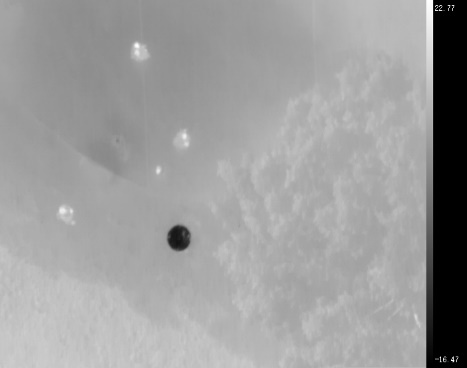
\includegraphics[height=4.27cm]{figures/4-1-红外图像左.jpg}
    \quad
    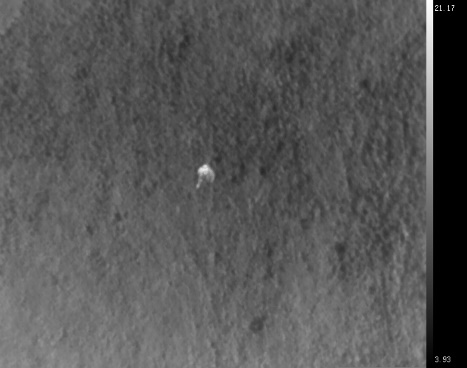
\includegraphics[height=4.27cm]{figures/4-1-红外图像右.jpg}
    \caption{阳光照射下热成像(左);无阳光照射热成像(右)}\label{hotImage}
\end{figure}

经过研究后发现,这层白雾向外所辐射的红外能量服从均匀分布。因此,可以对图像进行均值平移,滤除这层白雾。

设图像$\rm I$的长度为$\rm W$,宽度为$\rm H$,$P(x,y)$为位置$(x,y)$的灰度,$P'(x,y)$为均值平移后 $(x,y)$处的灰度值,则
\begin{equation}\label{平移}
P'(x,y)=P(x,y)-\frac{1}{WH}\sum_{i,j\in{W,H}} P(i,j)
\end{equation}
经过零均值化之后,有些像素点的灰度值会变为负数,因此需要进行归一化。这里采用灰度线性变换进行归一化。为了充分保留图像的细节,将归一化后每一帧红外图像的灰度都归一化到$0\sim255$的范围内。经过这样的处理,使得在不同的光照条件下,红外图像的灰度值都是基本相同的,为后面的进一步处理提供了方便。图\ref{hotImageResult}为上述处理的实验结果,可以看出,尽管光照强烈,但是经过处理之后,温度异常区域依然能够被有效的被提取出来。

\begin{figure}[h]
    \centering
    \begin{subfigure}[h]{0.3\textwidth}
        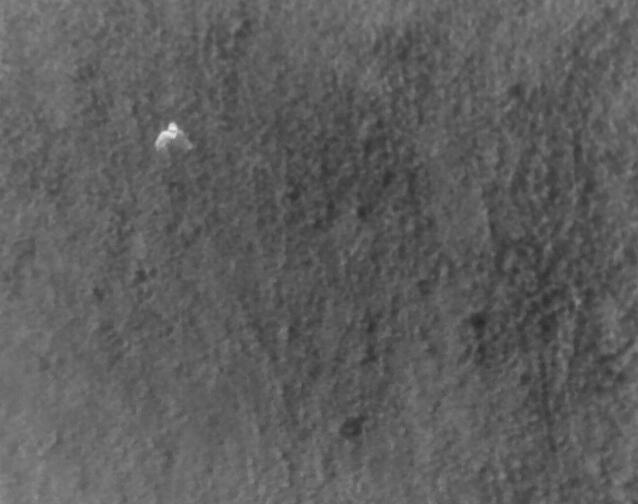
\includegraphics[width=\textwidth]{figures/红外图像预处理结果1.jpg}
    \end{subfigure}
    ~
    \begin{subfigure}[h]{0.3\textwidth}
        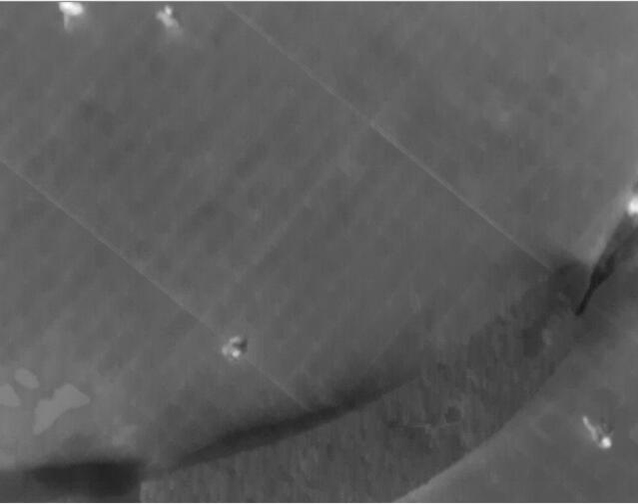
\includegraphics[width=\textwidth]{figures/红外图像预处理结果2.jpg}
    \end{subfigure}
    ~
    \begin{subfigure}[h]{0.3\textwidth}
        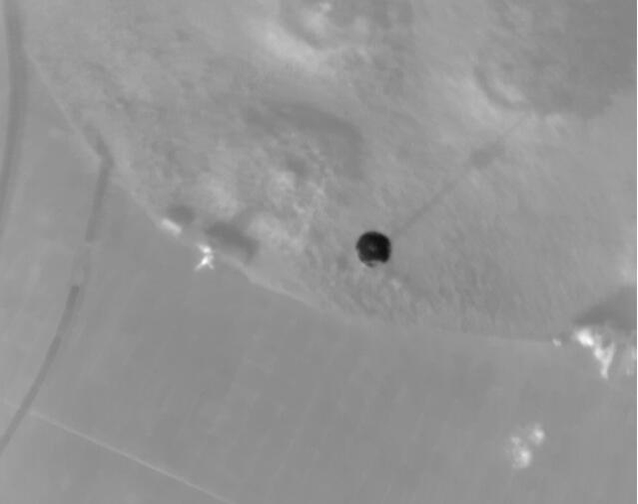
\includegraphics[width=\textwidth]{figures/红外图像预处理结果3.jpg}
    \end{subfigure}
    \vskip2ex
    \begin{subfigure}[h]{0.3\textwidth}
        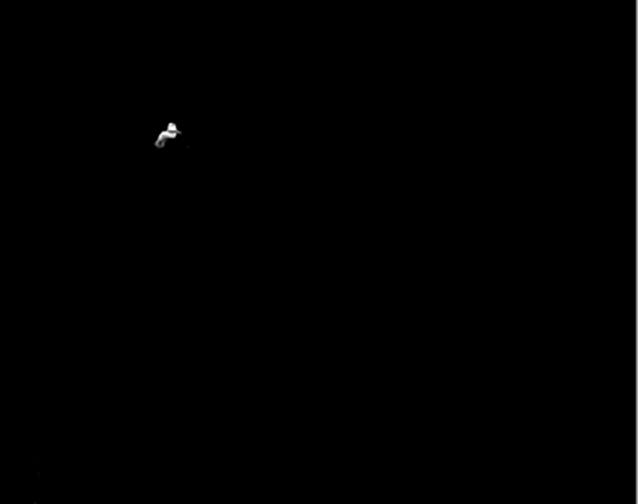
\includegraphics[width=\textwidth]{figures/红外图像预处理结果4.png}
    \end{subfigure}
    ~
    \begin{subfigure}[h]{0.3\textwidth}
        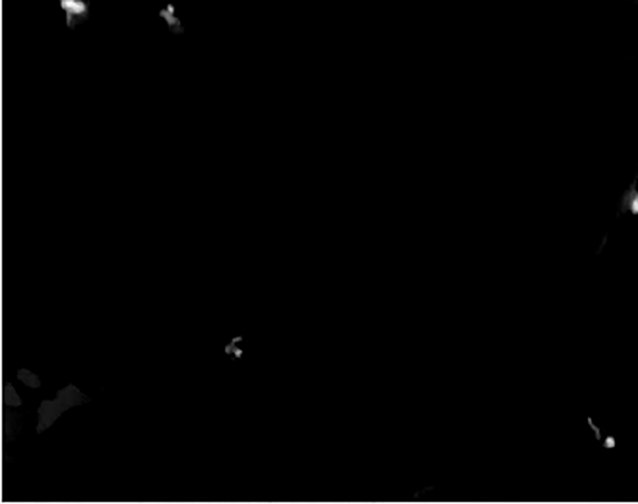
\includegraphics[width=\textwidth]{figures/红外图像预处理结果5.png}
    \end{subfigure}
    ~
    \begin{subfigure}[h]{0.3\textwidth}
        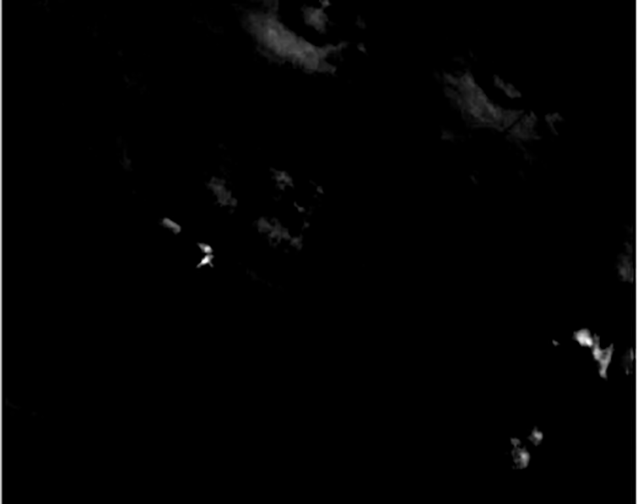
\includegraphics[width=\textwidth]{figures/红外图像预处理结果6.png}
    \end{subfigure}
    \caption{红外图像预处理结果(上为原图)}\label{hotImageResult}
\end{figure}

\noindent{\textbf{(3) 目标候选区域提取}}

由前面步骤已经可以得到噪点比较少的提取结果。然而,野外环境背景实在太复杂,并没有哪种算法能够完全准确的搜寻到目标。但是,可以通过先验知识,比如在飞行高度为$20m$的时候,目标的红外成像大小大约为$30\times30$个像素大小。过大或者过小的亮斑都极有可能是其他物体。因此通过判定连通域的面积大小,可以进一步剔除虚警。无人机搜救系统工作时,天空端的红外图像处理程序根据设置好的阈值,如果经过上述图像分析处理得到的目标框个数大于$0$,则无人机向地面发送报告指令,通知地面端采用光学检测手段进行光学搜索,同时将得到的目标候选包围框的坐标发送回地面端的计算设备。考虑到实际情况,即待搜救人员如果为多个,也不会分布的很分散,因此如果有多个目标,则候选目标区域为多个目标的最小外接矩形区域,如图\ref{hotImageROI}中的红色框所示区域。

\begin{figure}[h]
    \centering
    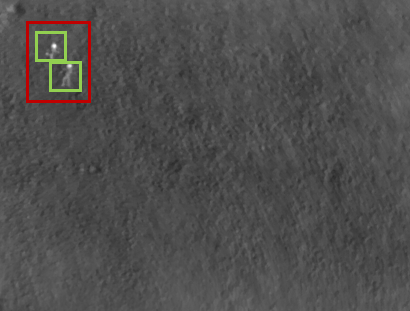
\includegraphics[width=5.61cm]{figures/红外图像目标候选区域.png}
    \caption{红外图像目标候选区域(红色)}\label{hotImageROI}
\end{figure}


地面端会在光学图像中选取对应的图像区域进行进一步的光学目标检测,同时,对应的光学区域将被高亮显示,方便地面工作人员进行人工同步的筛选。


\subsection{光学图像目标检测}

本系统面向的应用场景为野外搜救,野外环境复杂多变,同时,在无人机视角下,检测目标除了尺度会发生变化,形状,姿态也会发生较大的变化,如图4-4所示。经过大量相关实验,在这种场景下,传统的检测算法检测效果不是很理想,但是基于卷积神经网络DCNN(Deep Convolutional Neural Network)的检测算法能得到很好的检测结果。
\begin{figure}[h]
    \centering
    \begin{subfigure}[h]{0.3\textwidth}
        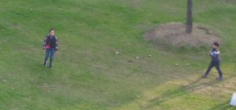
\includegraphics[width=\textwidth]{figures/目标示例样本1.png}
    \end{subfigure}
    ~
    \begin{subfigure}[h]{0.3\textwidth}
        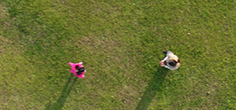
\includegraphics[width=\textwidth]{figures/目标示例样本2.png}
    \end{subfigure}
    ~
    \begin{subfigure}[h]{0.3\textwidth}
        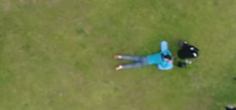
\includegraphics[width=\textwidth]{figures/目标示例样本3.png}
    \end{subfigure}
    \vskip1ex
    \begin{subfigure}[h]{0.3\textwidth}
        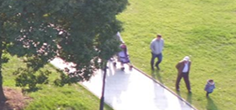
\includegraphics[width=\textwidth]{figures/目标示例样本4.png}
    \end{subfigure}
    ~
    \begin{subfigure}[h]{0.3\textwidth}
        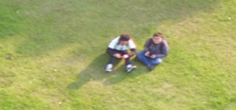
\includegraphics[width=\textwidth]{figures/目标示例样本5.png}
    \end{subfigure}
    ~
    \begin{subfigure}[h]{0.3\textwidth}
        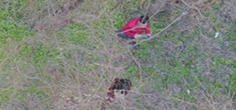
\includegraphics[width=\textwidth]{figures/目标示例样本6.png}
    \end{subfigure}

    \caption{各种姿态下, 不同相机视角下以及遮挡情况下的目标示例样本}\label{Samples}
\end{figure}

\noindent{\textbf{(1) UAV-PP无人机数据集}}

无人机视角下的人会存在各种姿态,经调查,目前比较流行的无人机数据集和通用数据集比如VOC、ImageNet都没有专门收录无人机视角下的人体姿态数据。针对基于DCNN的检测算法,为了得到更好的检测结果,需要先建立一个无人机视角下人的数据集。

本数据集采取VOC数据集格式,所建立的数据集称为(UAV perspective person dataset, UAV-PP)。UAV-PP数据集文件目录如图\ref{fold}所示。
\begin{figure}[h]
    \centering
    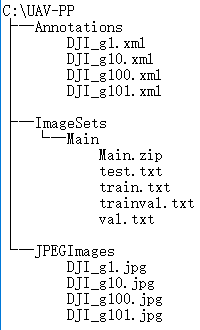
\includegraphics[width=4cm]{figures/目录结构.png}
    \qquad
    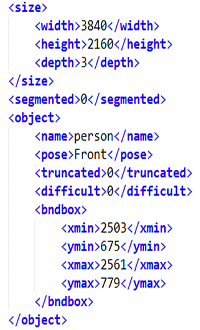
\includegraphics[width=4cm]{figures/标注示例.png}
    \caption{ UAV-PP 目录结构(左)以及标注示例(右)}\label{fold}
\end{figure}

其中,JPEGImages存放的是航拍图像。Annotation文件夹中存放的是JPEGImages中每一张图片对应的.xml格式标注文件,标注格式采用VOC格式,如图\ref{fold}右图所示。

\noindent{\textbf{(2) SSD检测算法}}

由于本系统需要实时地对无人机拍摄的图像进行处理,权衡检测速度和检测精度,基于DCNN的SSD(Single Shot MultiBox Detector)算法能满足本系统的需求。同时,为了更好的应用于本系统,我们使用上述自建数据集对原始SSD算法进行了微调,并应用于地面端进行光学图像处理。

SSD算法组合了多个不同层级不同分辨率下的feature map的预测结果来对抗目标的尺度变化。每个对象类别在每个默认框中的存在并且产生调整尺度变化大的物体检测。对于$300\times300$的输入图像,SSD可以在VOC2007数据集上以59FPS的速度达到74.3平均精度均值(Mean Average Precision, mAP),更精确版本使用$512\times512$大小的输入图像,可以达到76.9的mAP(均使用Nvidia TitanX显卡)。

SSD模型主要包含可以分为以下四个方面:
\begin{figure}[h]
    \centering
    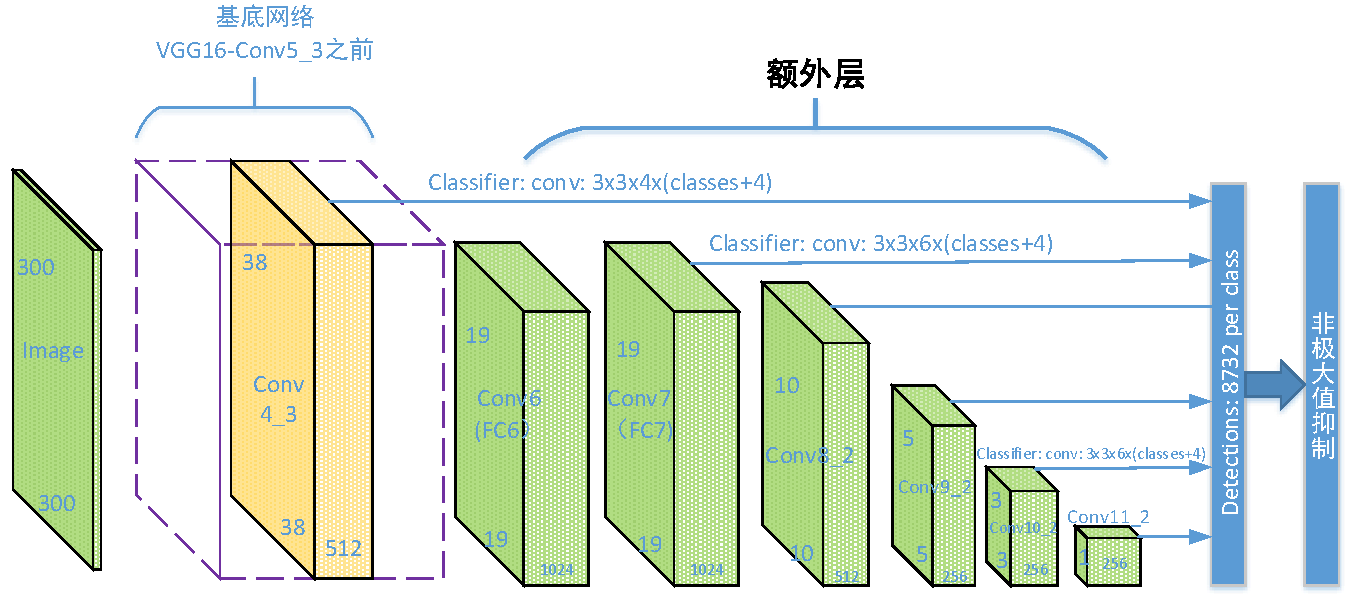
\includegraphics[width=14cm]{figures/SSD网络结构图.pdf}
    \caption{SSD 网络结构图}\label{SSDStruct}
\end{figure}


\begin{enumerate}[1)]
\item \textbf{基底网络。}截取当前流行的目标检测网络前面几个包含卷积核池化层用于做基底。
\item \textbf{多尺度特征图。}在基底网络的基础上,SSD算法在后面连接了多个卷积特征层。这些层的大小依次递减,这样就可以允许进行多尺度的检测。
\item \textbf{卷积检测预测器。}在基底网络后添加的每一个层可以利用卷积滤波器来生成一系列固定大小的预测结果。对于一个大小为$m\times n$的P通道的特征层,使用的是$3\times3$大小的核(kernel),产生的为该位置归属于某一个类别的得分,亦或是相对于默认bounding box的形状偏移量 。这样,在每一个$m\times n$大小的特征图位置上,kernel都会生成一个值。其中,形状偏移量是相对default bounding box与此时特征图上的位置的相对距离。
\item \textbf{默认bounding box和长宽比。}如图\ref{SSDBoundingBox}所示,在整个SSD网络的前面的多个特征图上,每一个特征图单元(cell)都会关联一系列默认的bounding box。每一个默认bounding box和cell之间的位置是固定的。对于每一个cell,给出它相对于cell中的默认bounding box的偏移量,以及这些默认框包含各类别物体的得分。具体来说,如果默认框为$K$个,则对于每个bounding box,在每个位置,要产生$C$个类别的分类得分以及$4$个相对偏移量(相对bounding box的$4$个顶点),所以一共需要$(C+4)\cdot{K}$个卷积核,对于$m\times n$大小的特征图输入,产生$Kmn\cdot{(C+4)}$大小输出特征图。
\end{enumerate}

\begin{figure}[h]
    \centering
    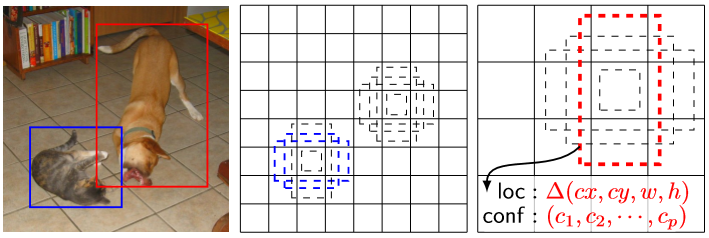
\includegraphics[height=3.5cm]{figures/SSD默认boundingbox.png}
    \caption{SSD默认boundingbox}\label{SSDBoundingBox}
\end{figure}

SSD框架虽然在VOC、COCO等数据集上获得了良好的表现,但是对于本系统的实际应用场景,仍需做进一步的调整与改进。针对自建数据集,SSD需要做一些参数的调整,主要是一些训练参数,比如学习率,冲量的调整,还包括Extra Network网络结构的微调,比如使用的卷积核的大小个数,以及网络最后输出层的输出类别数目。
由SSD模型的介绍可知,使用自建数据集实施检测任务的时候,可以从设计默认bounding box的分布入手。由于无人机视角的特殊性,目标的尺度变化不大,比较有限,因此,我们更改了尺度划分。此外,因为目标实际尺寸比较小,因此训练使用的batch大小从$128$适当增大到$512$。

另一方面,原始的SSD的基底网络是使用VGG16前面的预测层,一个$32\times32$的目标经过VGG后变成$2\times2$,这样就容易丢失后几层的语义信息。因此原始SSD对于小尺寸目标(如无人机视角下的人)的检测效果受到了影响。所以对于小目标检测,需要增加上下文的语义信息。经过研究,在神经网络中引入残差网络(Residual Network, ResNet)能够很好的保留目标语义信息。
\begin{figure}[h]
    \centering
    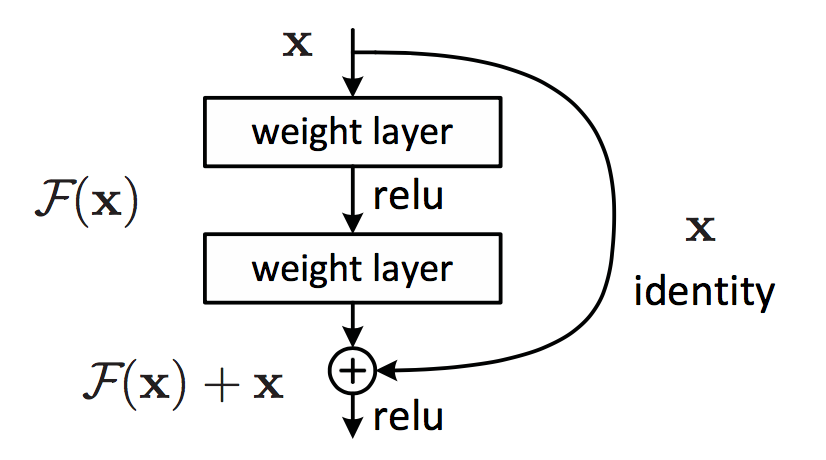
\includegraphics[height=3.5cm]{figures/ResNet.png}
    \caption{ResNet 基础结构}\label{ResNet}
\end{figure}
图\ref{ResNet}是ResNet的基础结构。ResNet在输出和输入之间引入一个shortcut connection,这样可以解决网络由于很深出现语义丢失的问题,从而可以把网络做的很深。综合考虑,本论文将使用深度适中的ResNet-101结构作为SSD的基底网络。



\section{无人机自主避障}

野外搜救无人机系统的工作环境是复杂多变的,这对于无人机的飞行安全是一个很大的考验。因此实现野外搜救无人机系统需要关注这一关键技术。本系统使用能得到图像的深度信息的双目相机来实现避障技术。

\subsection{使用双目视觉获取深度信息}

使用双目相机的一个好处就是可以根据左右两个相机的视差计算出物体的距离信息。
使用两个相机可以得到左右视图,两个视图必定产生差异,称之为“左右视差”,从左右视差(disparity)到“深度”(depth)的转换原理如图\ref{DoubleVision}所示。

\begin{figure}[hb]
    \centering
    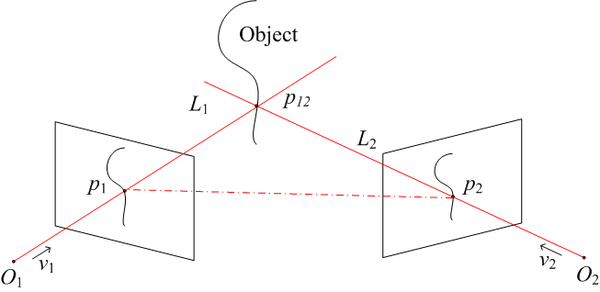
\includegraphics[height=4cm]{figures/双目视图测距原理.png}
    \caption{双目视图测距原理}\label{DoubleVision}
\end{figure}


设前方物体上的点$p_{12}$对应于左右视图上的点$p_1$和点$p_2$。则$p_1,p_2,p_{12}$构成一个三角形,通过求解这个三角形的各边长,顶点位置,就可以算出点$p_{12}$的坐标了,再进一步也就可以得到$p_{12}$的深度了。
由双目视图可以计算差异图,差异图重投影到3D就可以得到点云,如图\ref{3DCloud}所示。而点云数据恰好是对障碍信息一个最通用的描述。本系统采用的机器人操作系统ROS下,拥有的stero_image_pro节点,可以实现点云的获取。
 	 
\begin{figure}[h]
    \centering
    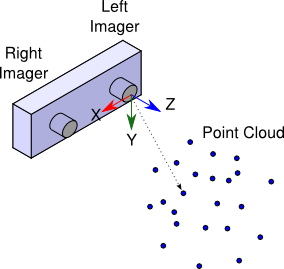
\includegraphics[height=4cm]{figures/3D点云.png}
    ~
    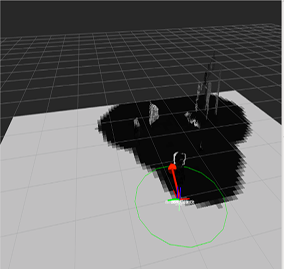
\includegraphics[height=4cm]{figures/点云可视化.png}
    \caption{3D点云(左); Guidance生成的点云可视化(右)}\label{3DCloud}
\end{figure}

图\ref{3DCloud}(右)是本系统根据Guidance双目视觉模块生成的3D点云图,得到的3D点云可以让无人机了解前方一定距离内的障碍信息,为避障提供条件。


\subsection{使用代价地图}

点云数据得到后,就可以得到障碍信息。首先,建立一个空的网格地图。在当前位置点,根据点云信息,有点云出现的位置设为Occupied,没有出现的位置设为Free,点云密度大于某个值的地方就认定为有固体障碍。通常使用基于代价地图的路径重规划躲避这些障碍。

代价地图分为全局代价地图和局部代价地图。由于本系统的应用场景是未知地图的巡航飞行,因此只能使用局部代价地图,这个是根据不断收到的传感器数据动态更新的地图。实际的避障中,首先需要初始化一个全局的规划器。这个全局规划器负责生成一个从指定的“起点”到指定的“目标点”之间的最短路径,这个生成的最短路径为最初状态的最佳路径。然后根据局部代价地图,局部规划器将根据最新的障碍信息不断调整更新最佳路径,并产生各个移动移动方向上的速度命令以便无人机避开障碍物。这些速度命令一般采用动态窗口方法来生成:
\begin{enumerate}[1)]
\item 在机器人控制空间$(dx,dy,d\theta)$中离散采样。
\item 对于每个采样速度,从机器人的当前状态执行正向仿真,以预测如果使用采样速度一段时间的运动会发生什么。
\item 使用包括诸如以下特征的度量来评估(打分)从正向模拟产生的每个轨迹:接近障碍物,接近目标,接近全局路径和速度。然后丢弃非法轨迹(与障碍物碰撞的轨迹)。
\item 选择最高得分的轨迹,并将相关速度发送到移动基地。
\item 清除得分并重复。

\begin{figure}[h]
    \centering
    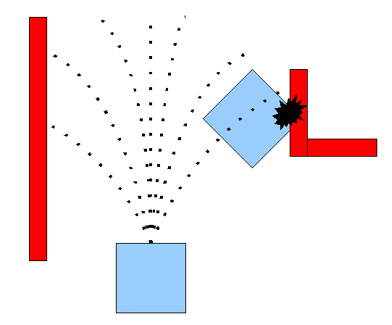
\includegraphics[height=4cm]{figures/局部规划器对正向模拟路径打分.png}
    \caption{局部规划器对正向模拟路径打分}\label{Grade}
\end{figure}

\end{enumerate}

在机器人操作系统ROS中,有专门的导航工具集成这些算法,只需要设法提供它所订阅的几个主题信息,它就会调用内部的全局规划器和局部规划器来生成系列的运动速度指令。然后无人机就可以按照传来的运动速度指令进行障碍躲避了。

\begin{figure}[h]
    \centering
    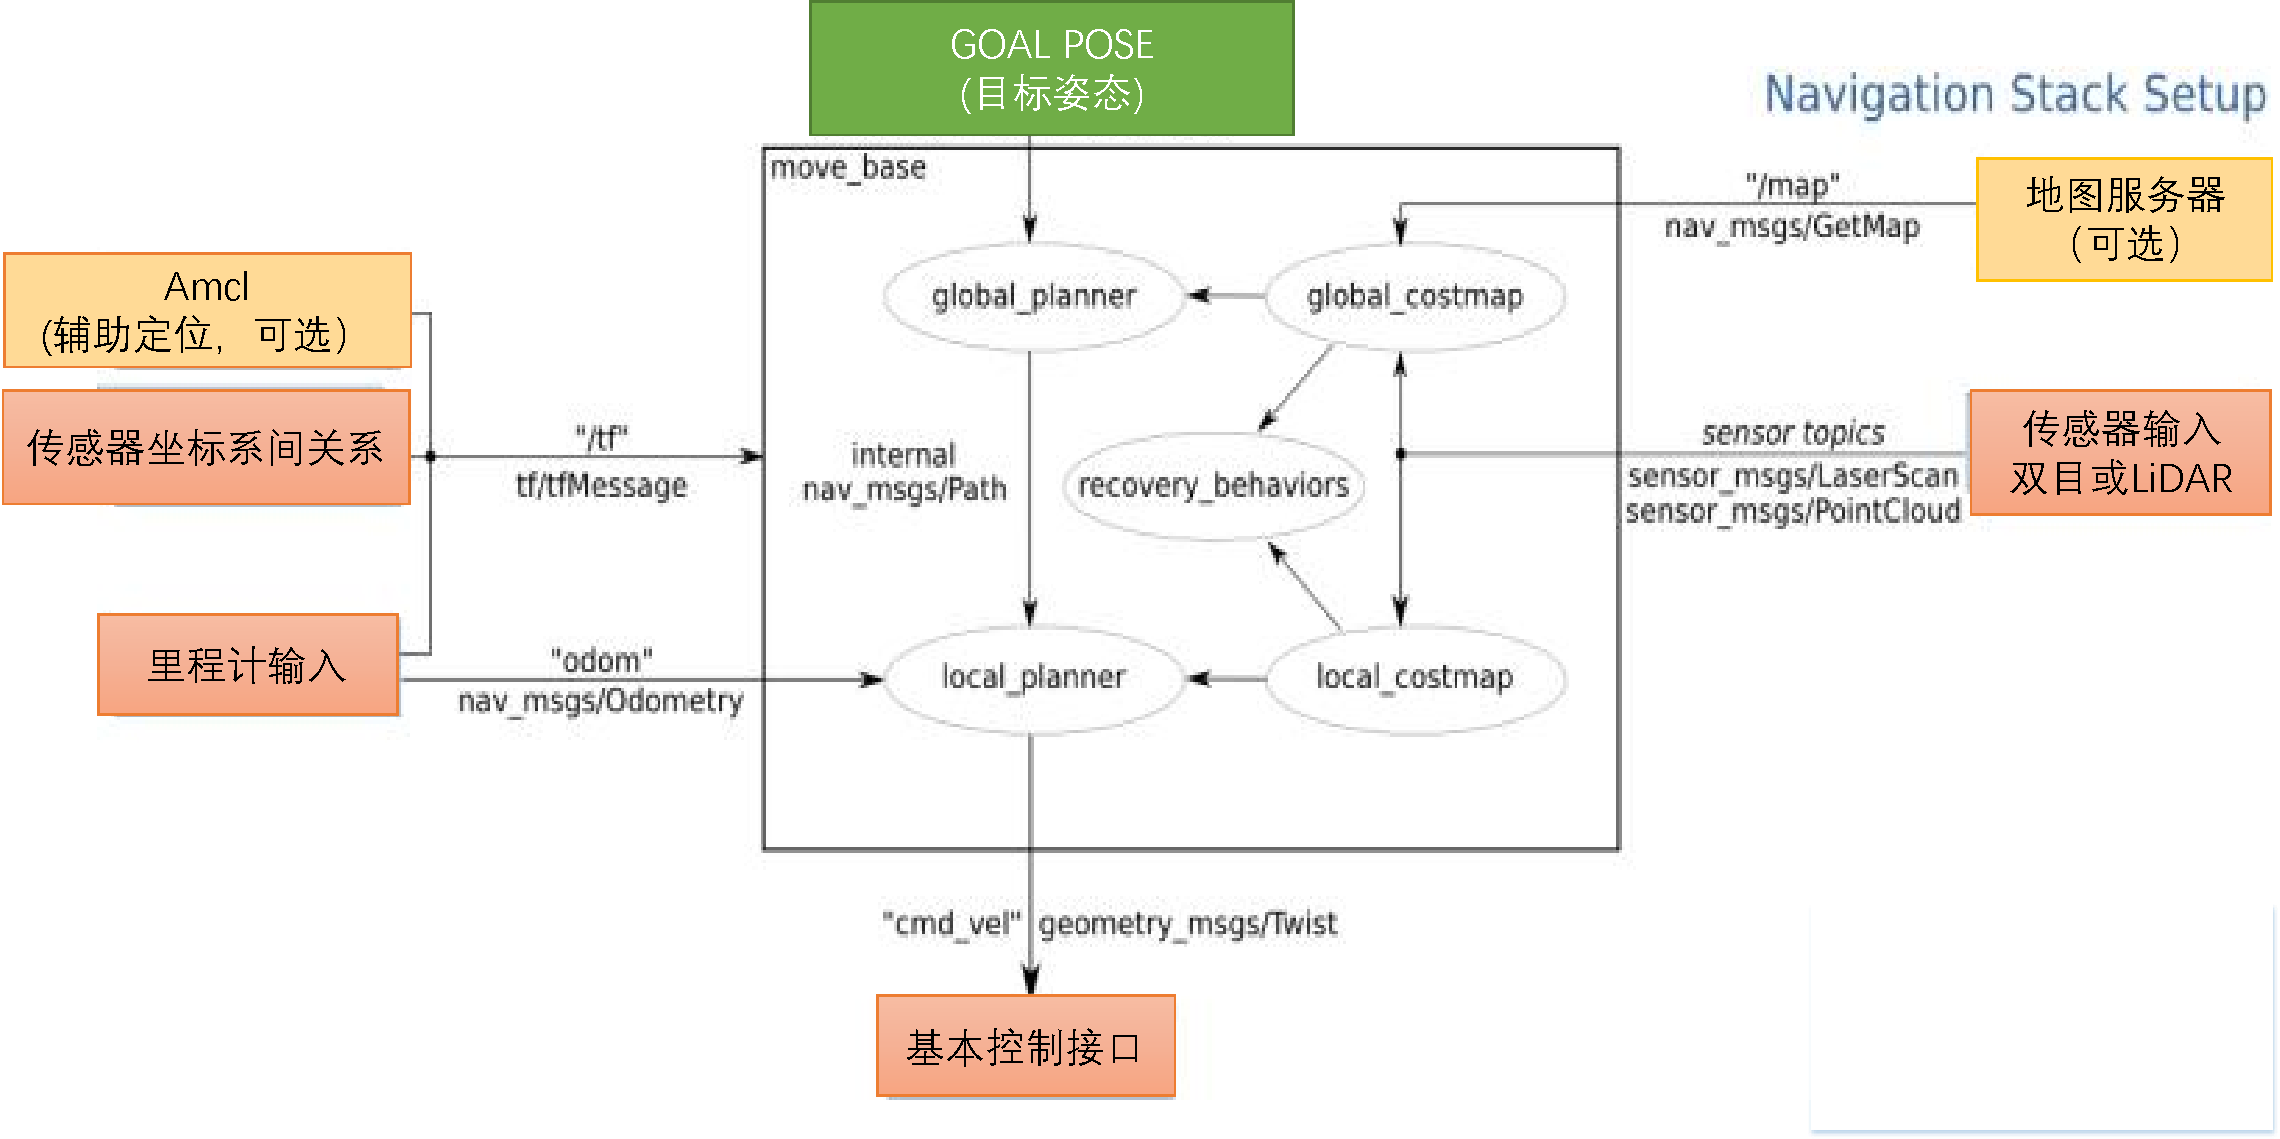
\includegraphics[width=13cm]{figures/ROS导航框图.pdf}
    \caption{ROS 导航框图}\label{ROS}
\end{figure}


\section{无人机自主移动降落}

本部分采用AprilTag视觉基准系统, 视觉基准系统通常指的是易于识别和彼此区分的人为标志。通过检测AprilTag,无人机将锁定降落位置点,并根据检测得到的AprilTag与无人机机身的相对6DOF(six degree of freedom)位姿来调整无人机的速度和姿态,最后实现精准移动降落。对于野外救援,并不能保证有平坦开阔的降落平台,这时可以在随行的汽车车顶上布置该视觉系统,引导无人机安全降落。

\subsection{AprilTag视觉基准系统}

本系统使用的AprilTag由两部分组成:标志检测器(Tag Detector)和编码系统(Coding System)。

因为视觉基准系统的意义主要是提供可靠的基准检测测试,因此需要精心设计。为了提高检测效率,AprilTag使用黑框将信息荷载包围住,以辅助精确定位。AprilTag内部的信息荷载只使用黑白块表示,且无任何对称性。AprilTag包含三个族,包括36h11,25h9,16h5。本系统使用25h9族。

\begin{figure}[h]
    \centering
    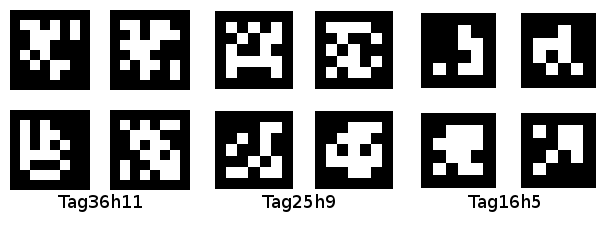
\includegraphics[height=5cm]{figures/各类AprilTag.png}
    \caption{各类 AprilTag}\label{ROS}
\end{figure}

\subsection{AprilTag检测}


AprilTag检测的第一步就是四边形的检测,因为已经使用了外围一圈黑框作定位辅助,因此四边形检测可以由以下几个步骤组成:
\begin{enumerate}[1)]
\item 将图像转换为灰度图像。
\item 图像滤波。

本部分使用高斯核大小为$3\times3$,标准差为$\sigma=0.8$的高斯滤波器。
\item 将灰度图二值化。

由于外围黑框的存在,因此使用正向二值化即可。

正向二值化的表达式如下:
\begin{equation}
    dst(x,y) = \left\{ 
    \begin{array}{ll}
        \max{Val} & \textrm{if $src(x,y)>T$;}\\
        0 & \textrm{其他;}
    \end{array} \right.
\end{equation}
其中$\max{Val}$为设定的规定值,$T$为二值化的阈值。

关于二值化的阈值,本部分使用的是局部自适应阈值算法,该方法根据局部像素块的像素值分布来确定该像素位置的二值化阈值$T$,从而使不同亮度、对比度以及纹理区域对应不同的二值化阈值,具有很好的鲁棒性。
\item 轮廓检测。

本部分采用的是OpenCV中的$findContours$函数。将上述得到的二值图像作为输入,可以得到一幅图像中存在的所有轮廓。由于我们需要的仅仅是四边形的轮廓,因此需要对得到的轮廓进行多边形拟合,使用OpenCV中的$approxPolyDP$函数即可完成。该函数将对输入的一组轮廓进行多边形拟合,通过判断拟合得到的多边形的顶点个数是否为$4$就可以筛选出候选轮廓。

\item 候选区域筛选

由于标志内部仍可能被检测出四边形轮廓,因此,需要判定得到的四边形是否为最外围的边界框。由于实际操作中,标志的尺寸是已知的,无人机飞行的高度和相机成像分辨率也是已知的,这样就可以得到标志占据画面的比例大小来进一步筛选。对于每个候选的拟合得到的四边形,计算其相邻顶点之间的距离:
\begin{equation}
dist_{ij}=(x_i-x_j)^2+(y_i-y_j)^2
\end{equation}
其中,$i,j$为相邻的两个顶点,若满足$\min{dist_{ij}}>\varepsilon$则保留该四边形,$\varepsilon$为设定的阈值,此处为$5000$。
\end{enumerate}

\begin{figure}[h]
    \centering
    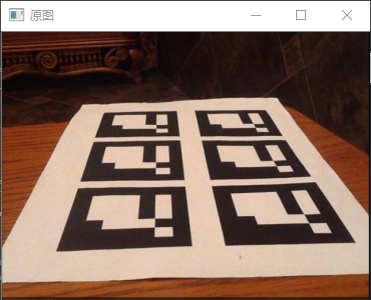
\includegraphics[height=4cm]{figures/检测结果1.png}
    \quad
    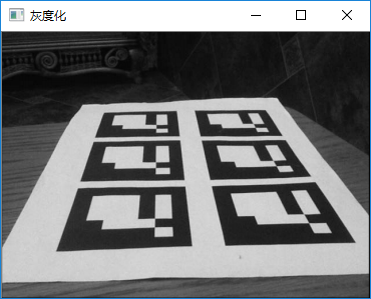
\includegraphics[height=4cm]{figures/检测结果2.png}
    \vskip1ex
    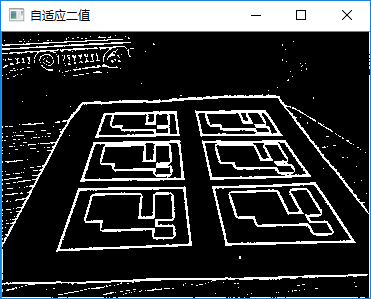
\includegraphics[height=4cm]{figures/检测结果3.png}
    \quad
    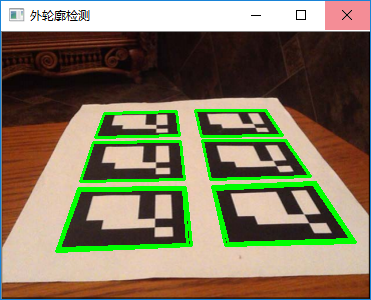
\includegraphics[height=4cm]{figures/检测结果4.png}
    \caption{检测结果:原图(左上)灰度图(右上)二值化(左下)外轮廓检测(右下)}\label{DetectResult}
\end{figure}

\subsection{AprilTag识别}

AprilTag系统中,每个标志可以划分为$7\times7$个细胞单元,黑色格子代表$0$,白色格子代表$1$。则标志内部可以由5个5bit的01字符串表示(除去外围的$2$个格子)。接下来将采用海明码编码。5bit中的3bit用于校验,2bit用于存放数据,则每个标志可以表示$4^5=1024$个数据。引入编码系统,是为了提高纠错能力以及进一步筛除虚警。

\begin{figure}[h]
    \centering
    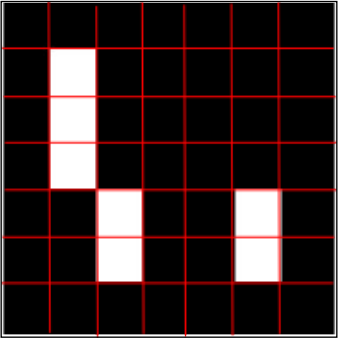
\includegraphics[height=4cm]{figures/AprilTagCell.png}
    \caption{AprilTag划分cell单元}\label{AprilTagCell}
\end{figure}

对于海明编码,如果待检测的二进制码为$n$,若要求纠错能力,则需设置$k$位校验码,并且满足$2^k≥n+k+1$,即$k$个校验码需要涵盖$n$位数据码以及自身$k$位校验码任意一位出错或者全部正确$+1$的情况。因此,对于AprilTag系统,需要$k=3$。校验码设为$c_1,c_2,c_3$,将其从左往右间插在第$2^i$的位置,所以一个AprilTag可以编码表示为$c_1c_2b_1c_3b_2$,$b_1,b_2$为信息码。

根据海明编码规则,$c_1$负责校验码字(包括信息码和校验码)的第$1,3,5$位; $c_2$负责校验码字的第$2,3$位, $c_3$负责校验第$4,5$位。若采用偶校验(即被校验的位加上自身一共有偶数个“1”),则$c_3=b_2$。
	
有了海明编码,在检测到候选目标区域四边形后,就可以通过解码的方式来判定其是否为定义的标志了,这样则大大降低了虚警,同时由于有纠错能力,也有着较好的鲁棒性。

根据海明编码,下面将确定标志ID。

由于AprilTag可以看出一个编码系统,因此每个标志可以給它编定一个ID号码。主要有下面三步:
\begin{enumerate}[1)]
\item 根据得到的四边形顶点进行反透视变换,将四边形还原为正方形。
\item 对候选区域使用大津阈值二值化,并归一化大小,比如$100\times100$。
\item 解码识别标志。

将$100$像素$\times$$100$像素划分为$7\times7$的cell,计算轮廓cell(外围一圈)中非零像素个数,若大于cell中的所有像素个数一半,则认为是"白"格,该轮廓被认定为不完整,舍弃之。

然后,识别将剩余的$5\times5$个cell大小的编码区域并根据海明编码规则进行编码,存入矩阵bitMatrix。

由于得到的bitMatrix有可能是旋转后的结果,因此还需要找到具体旋转了多少角度。具体来说,因为每一行5bit码中有两个bit的信息码,因此共有4种编码可能(每一行)。对bitMatrix的每一个旋转状态(每旋转$90^\circ$为一个状态),对bitMatrix中的每一行,寻找其与这四种可能编码的海明距离(即不同值个数)中最小值,四个最小值之和为该旋转状态下的海明距离。可以通过求四个状态下海明距离的最小值来得到标志的旋转状态。最后,一个标志的编码,和顶点顺序都确定下来了。
\end{enumerate}




\subsection{相机三维姿态解算}

为了引导无人机进行姿态调整,最后降落在标志上,在识别了标志之后,需要解算出标志相对于相机的姿态。在相机坐标系中的点$P_c(x_c,y_c,z_c)$。可以由对应的世界坐标系统中的点$P_w(x_w,y_w,z_w)$通过一个旋转变换$R(3\times3)$和一个平移变换$T(3\times1)$得到:
\begin{equation}
P_c=RP_w+T
\end{equation}
写成齐次式为:
\begin{equation}\label{齐次式}
\begin{pmatrix}
x_c \\
y_c \\
z_c \\
1    \end{pmatrix} = \begin{pmatrix}
R & T\\
0_3^T & 1 \end{pmatrix}
\begin{pmatrix}
x_w \\
y_w \\
z_w \\
1    \end{pmatrix}
\end{equation}
根据透视投影模型:
\begin{figure}[h]
    \centering
    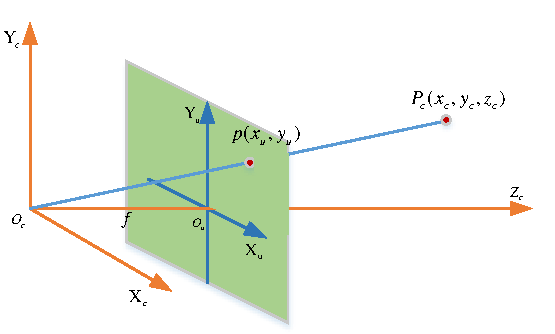
\includegraphics[height=5cm]{figures/透视投影模型.pdf}
    \caption{透视投影模型}\label{透视投影模型}
\end{figure}
 
\begin{equation}
x_u=f\frac{x_c}{z_c} \qquad y_u=f\frac{y_c}{z_c}
\end{equation}
$x_u,y_u$ 为成像系统感光器件(图像的实际物理)坐标系。则公式\ref{齐次式}化为:
\begin{equation}
z_c\begin{pmatrix}
x_u \\
y_u \\
1    \end{pmatrix} = \begin{pmatrix}
f & 0 & 0 & 0\\
0 & f & 0 & 0\\
0 & 0 & 1 & 0\end{pmatrix}
\begin{pmatrix}
x_c \\
y_c \\
z_c \\
1    \end{pmatrix}
\end{equation}
又因为相机物理尺寸坐标系和图像坐标系之间有如下关系:
\begin{equation}
\begin{pmatrix}
u \\
v \\
1    \end{pmatrix} = \begin{pmatrix}
1/d_x & 0 & u_0\\
0 & 1/d_y & y_0\\
0 & 0 & 1\end{pmatrix}
\begin{pmatrix}
x_u \\
y_u \\
1 \end{pmatrix}
\end{equation}
其中 $d_x,d_y$ 为图像中每个像素分别在 $u,v$ 中上对应的实际物理尺寸,单位为$m/pixel$。由此可以得到图像坐标系到世界坐标系的转换关系:
\begin{equation} 
\begin{split}
    z_c\begin{pmatrix}
u \\
v \\
1    \end{pmatrix} &= \begin{pmatrix}
1/d_x & 0 & u_0\\
0 & 1/d_y & y_0\\
0 & 0 & 1\end{pmatrix}
\begin{pmatrix}
f & 0 & 0 & 0 \\
0 & f & 0 & 0 \\
0 & 0 & 1 & 0 \end{pmatrix}
\begin{pmatrix}
R & T \\
0^T & 1 \end{pmatrix}
\begin{pmatrix}
x_w \\
y_w \\
z_w \\
1    \end{pmatrix} \\
&=\begin{pmatrix}
\alpha & 0 & u_0 & 0 \\
0 & \beta & v_0 & 0 \\
0 & 0 & 1 & 0 \end{pmatrix}
\begin{pmatrix}
R & T \\
0^T & 1 \end{pmatrix}
\begin{pmatrix}
x_w \\
y_w \\
z_w \\
1    \end{pmatrix} \\
&= M_1M_2\overrightarrow{X_w}
\end{split}
\end{equation}

其中$M_1$称为相机的内参数,是每个相机出厂之时就已经决定好的。可以通过各种相机标定算法标定得到。而 $M_2$就是需要的外参数,其包含了旋转矩阵和平移矩阵。$M_1,M_2$都得到之后,便可求出相机相对物体(世界坐标系)的姿态了。求解$M_2$是一个Perspective-n-points(PnP)问题。OpenCV中可以由solvePnP函数计算得到。因为AprilTag为平面标志,因此可令$z_c=0$,并以AprilTag标志的左上角为世界坐标系原点,则可以唯一确定相机相对于标志的位姿了。

\begin{figure}[h]
    \centering
    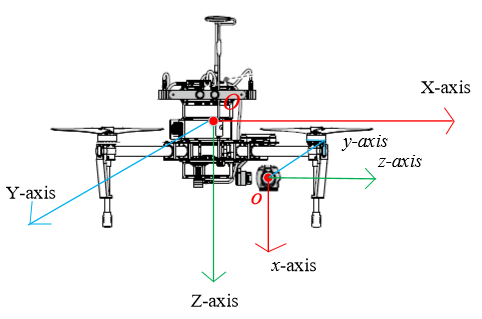
\includegraphics[height=5cm]{figures/无人机坐标系与相机坐标系.png}
    \caption{无人机坐标系与相机坐标系}\label{Axis}
\end{figure}

图\ref{Camera}为解算出来的相机的位姿。

\begin{figure}[htb]
    \centering
    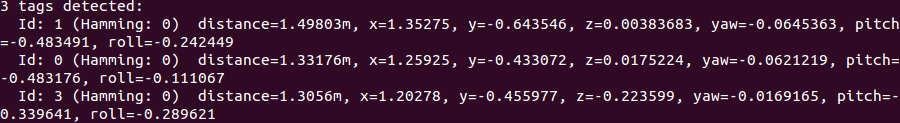
\includegraphics[width=13cm]{figures/相机姿态估计结果.png}
    \caption{相机姿态估计结果}\label{Camera}
\end{figure}
